\subsubsection{19.12.14}
\begin{enumerate}
	\item Время начала и окончания собрания: 16:00 - 20:00.
	\item Цели собрания:
	\begin{enumerate}
		\item Проверить и корректировать контакты на драйверах моторов.
		
		\item Сделать заготовку для нового ковша.
		
	\end{enumerate}
	
	\item Проделанная работа:
	\begin{enumerate}
		\item Была откорректирована длина неизолированной части проводов, соединяющих драйвера с аккумулятором, так, чтобы они не могли замкнуться друг на друге. В дальнейшем необходимо запаять конщы этих проводов. Сегодня этого сделать не удалось из-за отсутствия паяльника.
		
		\item Была вырезана заготовка для нового ковша. В дальнейшем планируется скрепить ковш степлером. 
		
		\begin{figure}[H]
			\begin{minipage}[h]{0.2\linewidth}
				\center  
			\end{minipage}
			\begin{minipage}[h]{0.6\linewidth}
				\center{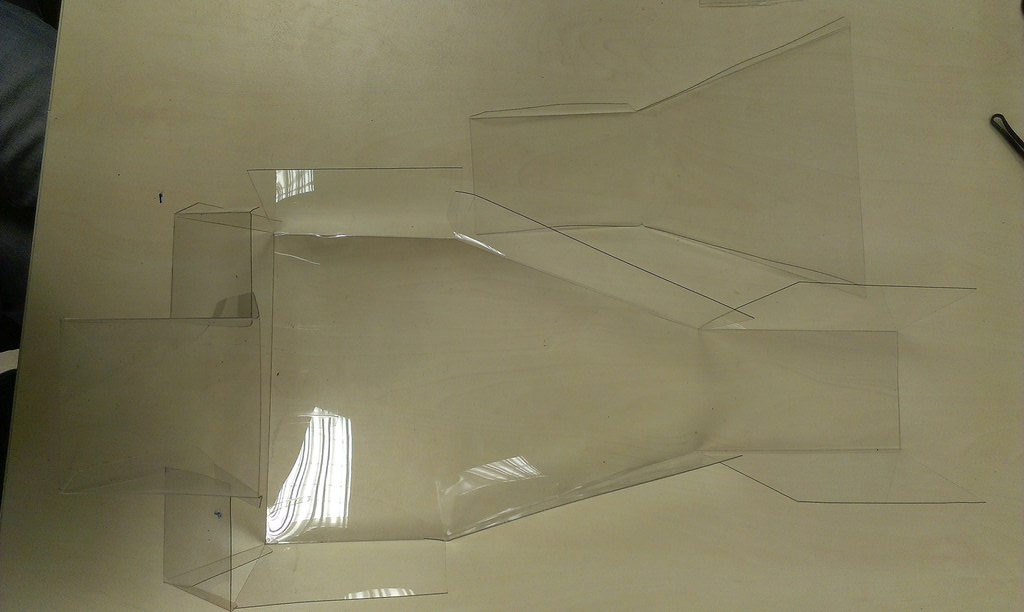
\includegraphics[scale=0.25]{days/19.12.14/images/01}}
				\caption{Заготовка ковша}
			\end{minipage}
		\end{figure}
		
	\end{enumerate}
	\item Итоги собрания:
	\begin{enumerate}
		\item Контакты на драйверах откорректированы по длине, но не запаяны.
		
		\item Сделана заготовка для нового ковша.
		

	\end{enumerate}
	
	\item Задачи для последующих собраний:
	\begin{enumerate}
		\item Запаять концы проводов, соединяющих аккумулятор с драйверами.
		
		\item Скрепить степлером новый ковш.
		
	\end{enumerate}
	
\end{enumerate}
\fillpage